\documentclass{article}
\usepackage{tikz}

\title{Structural dynamics problems}
\author{J. Bonet, M. Masó, R. Chacón}
\date{July 1, 2022}

\newenvironment{problem}[1]{
    \begin{minipage}{\textwidth}
    {\bfseries Problem #1}   
}{
    \end{minipage}
}

\begin{document}

\maketitle

\section{Problems}

\subsection{Free vibration of SDOF structures}

\begin{problem}{1}
For the structures shown, determine the natural frequency of vibration using simple structural concepts.

\begin{center}
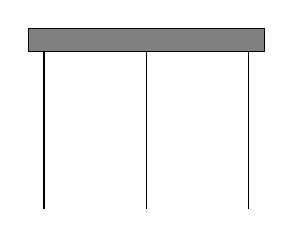
\begin{tikzpicture}
    \draw[fill=gray] (0,2) rectangle (3,2.3);
    \draw (0.2,0) -- (0.2,2);
    \draw (1.5,0) -- (1.5,2);
    \draw (2.8,0) -- (2.8,2);
\end{tikzpicture}
\hfill
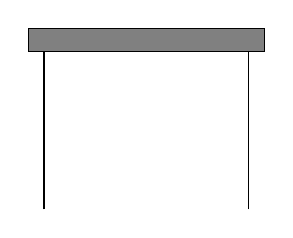
\begin{tikzpicture}
    \draw[fill=gray] (0,2) rectangle (3,2.3);
    \draw (0.2,0) -- (0.2,2);
    \draw (2.8,0) -- (2.8,2);
\end{tikzpicture}
\hfill
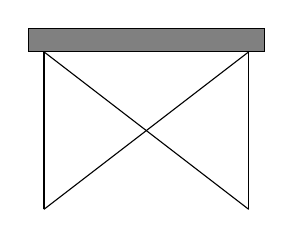
\begin{tikzpicture}
    \draw[fill=gray] (0,2) rectangle (3,2.3);
    \draw (0.2,0) -- (0.2,2);
    \draw (2.8,0) -- (2.8,2);
    \draw (0.2,0) -- (2.8,2);
    \draw (0.2,2) -- (2.8,0);
\end{tikzpicture}
\end{center}
\end{problem}

\begin{problem}[2]
For the structures shown, determine the natural frequency of vibration using Rayleigh's method.
\end{problem}

\section{Answers}

\end{document}
